\section{Preliminaries}
\label{sec:prelim}

In this section some background knowledge will be presented in order to understand our work. For a detailed explaination the interested reader is suggested to have a look at the cited papers. 
\subsection{Declarative Programming and Prolog}
The guiding principle of declarative programming is 
\[ALGORITHM = LOGIC + CONTROL.\]
Prolog is the first declarative programming language emerged by this principle. Computation in Prolog is done by use of recursion. Solutions are obtained by means of SLD-resolution and unification. As an example, a simple Prolog program \(P_1\) that  is able to append two list and to compute correctly the reversion of a list can be: 
\begin{align}
append ([\:], X, X).& \\
append ([X|Y], Z, [X|T ]) &\leftarrow append (Y, Z, T ). \\
reverse([ ], [ ]).&\\
reverse([X|Y ], Z) &\leftarrow append (U, [X], Z), reverse(Y, U ). \label{eq:1}
\end{align}
where [*|*] is a list contructor (an high order contructor).
If we wrote the following rule 
\begin{align}
reverse([X|Y ], Z) \leftarrow reverse(Y, U ), append(U, [X], Z). \label{eq:2}
\end{align}

instead of the rule number \ref{eq:1} in program \(P_1\), the meaning of the rule would not change but something unexpected happens dring the computation. Indeed the function reverse does not terminate because Prolog, due to the SLD-derivation, will call the reverse predicate endlessly. Moreover if we consider the program  \(P_2\):
\begin{align}
pig((88,34)).& \\
easy\_taget(X) &\leftarrow pig(X), not\: difficult\_taget(X). \\ 
difficult\_taget(X) &\leftarrow pig(X), not\: easy\_taget(X) 
\end{align}
it is easy to conclude that also this program will not terminate even if we know that the intuitive models are \(\{pig((88,34)), difficult\_taget((88,34))\}\) or \\ \(\{pig((88,34)), easy\_taget((88,34))\}\).

This problem force the programmer to think about what the engine prolog does in order to compute a solution but this is not in accordance to what the guiding principle of declarative programming states.
Indeed, it is desirable that
\begin{enumerate}
\item the order of program rules does not matter
\item the order of subgoals in a rule body does not matter.
\end{enumerate}


\subsection{Stable Model Semantics}
Stable Models of a logic program \(P\) are models of \(P\) and they enjoy many properties which reflect natural intuitions. Indeed  Stable Models help us to find the intuitive model of the modified program \(P_1\) and \(P_2\). The idea is guessing an interpretation of the program, and test its satisfiability. In order to do so, the program from which the model is wanted to be found is first reducted. The algoritm for program reduction is:

Given a program P and an interpretation M , \(P_M\) is a program obtained by 
\begin{enumerate} 
\item removing rules with not a in the body for each \(a \in M\)
\item removing literals not a from all other rules
\end{enumerate}
After the reduction phase the least model \(LM(P_M)\) of \(P_M\) is computed and it is tested if \(M = LM(P_M)\). If the equality holds M is called a Stable Model of \(P\).

if we consider again the program \(P_2\), we could have the following reasonable interpretations.
\begin{align*}
M_1&= \{pig((88,34)), easy\_taget((88,34))\}  \\
M_2&= \{pig((88,34)), difficult\_taget((88,34))\} \\
M_3&= \{pig((88,34)), easy\_taget((88,34)), difficult\_taget((88,34))\} \\
M_4&= \{pig((88,34))\}
\end{align*}

by the definitions stated above it is easy to check that only M1 and M2 are stable models. IF THERE IS SPACE I WILL EXPLAIN THIS STATEMENT


\subsection{Answer Set Programming}

ASP \cite{} is a declarative programming language capable of overcoming the limitations of Prolog in the programs \(P_1\) and \(P_2\). Its basic idea is:
\begin{enumerate}
\item expressing the problem and represent it with a logic program in such a way that models of the logic program are solutions for the problem.
\item using some AS solver in order to compute some model of the program
\item extract a solution for the problem from the model of the program
\end{enumerate}
as shown in Figure \ref{fig:ASP1}.
\begin{figure}
  % FIXME: f1.png not checked in.
  %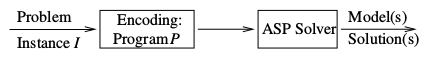
\includegraphics[width=\linewidth]{f1.png}
  \caption{logical steps made in order to find a stable model of a program.}
  \label{fig:ASP1}
\end{figure}
 
Traditional answer set solvers typically have a two level architecture:
\begin{enumerate}
\item Grounding Step: Given a program \(P\) with variables, a (subset) \(P'\) of its grounding is generated which has the same answer sets as \(P\) .
\item Model Search: The answer sets of the grounded (propositional) program \(P'\) are computed.
\end{enumerate}

There are different techniques for each of the two steps described and their presentation is out of the scope of this paper. For a more detailed explaintion \cite(bho).

\subsection{Hex Programs}
HEX programs \cite{} were introduced as a generalization of  extended logic programs under the answer set semantics. The syntax of HEX programs extend ordinary ASP programs by external atoms, which enable a bidirectional interaction between a program and external sources of computation. External atoms have a list of input parameters (terms or predicate names) and a list of output parameters. Informally, to evaluate an external atom, the reasoner passes the terms and extensions of the predicates in the input tuple to the external source associated with the external atom. The external source computes output tuples that are matched with the output list. Formally, an external atom is of the form \(\&g\:[Y]\:(X)\), where \(Y = Y_1, \dotso , Y_k\) are input parameters the set of terms, variables and predicates and \(X = X_1, \dotso , X_l \) are output terms. 

